\begin{landscape}
\subsection{\centering Attorney Information}
\begin{table}[H]
    \centering
    \renewcommand{\arraystretch}{1} % Add space between rows
    \caption{Attorney Summary (1-25)}
    \vspace{2mm}
    \csvreader[
        tabular= {cccccc},
        table head = {
            \toprule
            \footnotesize Attorney &
            \footnotesize Firm/Office &
            \footnotesize Law School &
            \footnotesize SCOTUS Clerkship &
            \footnotesize Prior Appearances &
            \footnotesize Previous Cases \\
            \midrule
        },
        table foot = \bottomrule
    ]{"Statpack Replication Data/Oral Arguments/Attorney Information/attorney_summary_stats_1.csv"}{}%
    {\footnotesize\csvcoli & \footnotesize\csvcolii & \footnotesize\makecell{\csvcoliii} & \footnotesize\csvcoliv & \footnotesize\csvcolv & \footnotesize\csvcolvi}
    \label{tab:table1}
\end{table}
\end{landscape}

\newpage

\begin{landscape}
\begin{table}[H]
    \centering
    \renewcommand{\arraystretch}{1} % Add space between rows
    \caption{Attorney Summary (26-50)}
    \vspace{2mm}
    \csvreader[
        tabular= {cccccc},
        table head = {
            \toprule
            \footnotesize Attorney &
            \footnotesize Firm/Office &
            \footnotesize Law School &
            \footnotesize SCOTUS Clerkship &
            \footnotesize Prior Appearances &
            \footnotesize Previous Cases \\
            \midrule
        },
        table foot = \bottomrule
    ]{"Statpack Replication Data/Oral Arguments/Attorney Information/attorney_summary_stats_2.csv"}{}%
    {\footnotesize\csvcoli & \footnotesize\csvcolii & \footnotesize\makecell{\csvcoliii} & \footnotesize\csvcoliv & \footnotesize\csvcolv & \footnotesize\csvcolvi}
    \label{tab:table1}
\end{table}
\end{landscape}

\newpage

\begin{landscape}
\begin{table}[H]
    \centering
    \renewcommand{\arraystretch}{1} % Add space between rows
    \caption{Attorney Summary (51-75)}
    \vspace{2mm}
    \csvreader[
        tabular= {cccccc},
        table head = {
            \toprule
            \footnotesize Attorney &
            \footnotesize Firm/Office &
            \footnotesize Law School &
            \footnotesize SCOTUS Clerkship &
            \footnotesize Prior Appearances &
            \footnotesize Previous Cases \\
            \midrule
        },
        table foot = \bottomrule
    ]{"Statpack Replication Data/Oral Arguments/Attorney Information/attorney_summary_stats_3.csv"}{}%
    {\footnotesize\csvcoli & \footnotesize\csvcolii & \footnotesize\makecell{\csvcoliii} & \footnotesize\csvcoliv & \footnotesize\csvcolv & \footnotesize\csvcolvi}
    \label{tab:table1}
\end{table}
\end{landscape}

\newpage

\begin{landscape}
\begin{table}[H]
    \centering
    \renewcommand{\arraystretch}{1} % Add space between rows
    \caption{Attorney Summary (76-102)}
    \vspace{2mm}
    \csvreader[
        tabular= {cccccc},
        table head = {
            \toprule
            \footnotesize Attorney &
            \footnotesize Firm/Office &
            \footnotesize Law School &
            \footnotesize SCOTUS Clerkship &
            \footnotesize Prior Appearances &
            \footnotesize Previous Cases \\
            \midrule
        },
        table foot = \bottomrule
    ]{"Statpack Replication Data/Oral Arguments/Attorney Information/attorney_summary_stats_4.csv"}{}%
    {\footnotesize\csvcoli & \footnotesize\csvcolii & \footnotesize\makecell{\csvcoliii} & \footnotesize\csvcoliv & \footnotesize\csvcolv & \footnotesize\csvcolvi}
    \label{tab:table1}
\end{table}
\end{landscape}


\newpage

\begin{landscape}
\centering
\vspace*{\fill}

\begin{multicols}{3}

    \begin{figure}[H]
        \centering
        \caption{SCOTUS Clerkship}
        \vspace{2.5mm}
        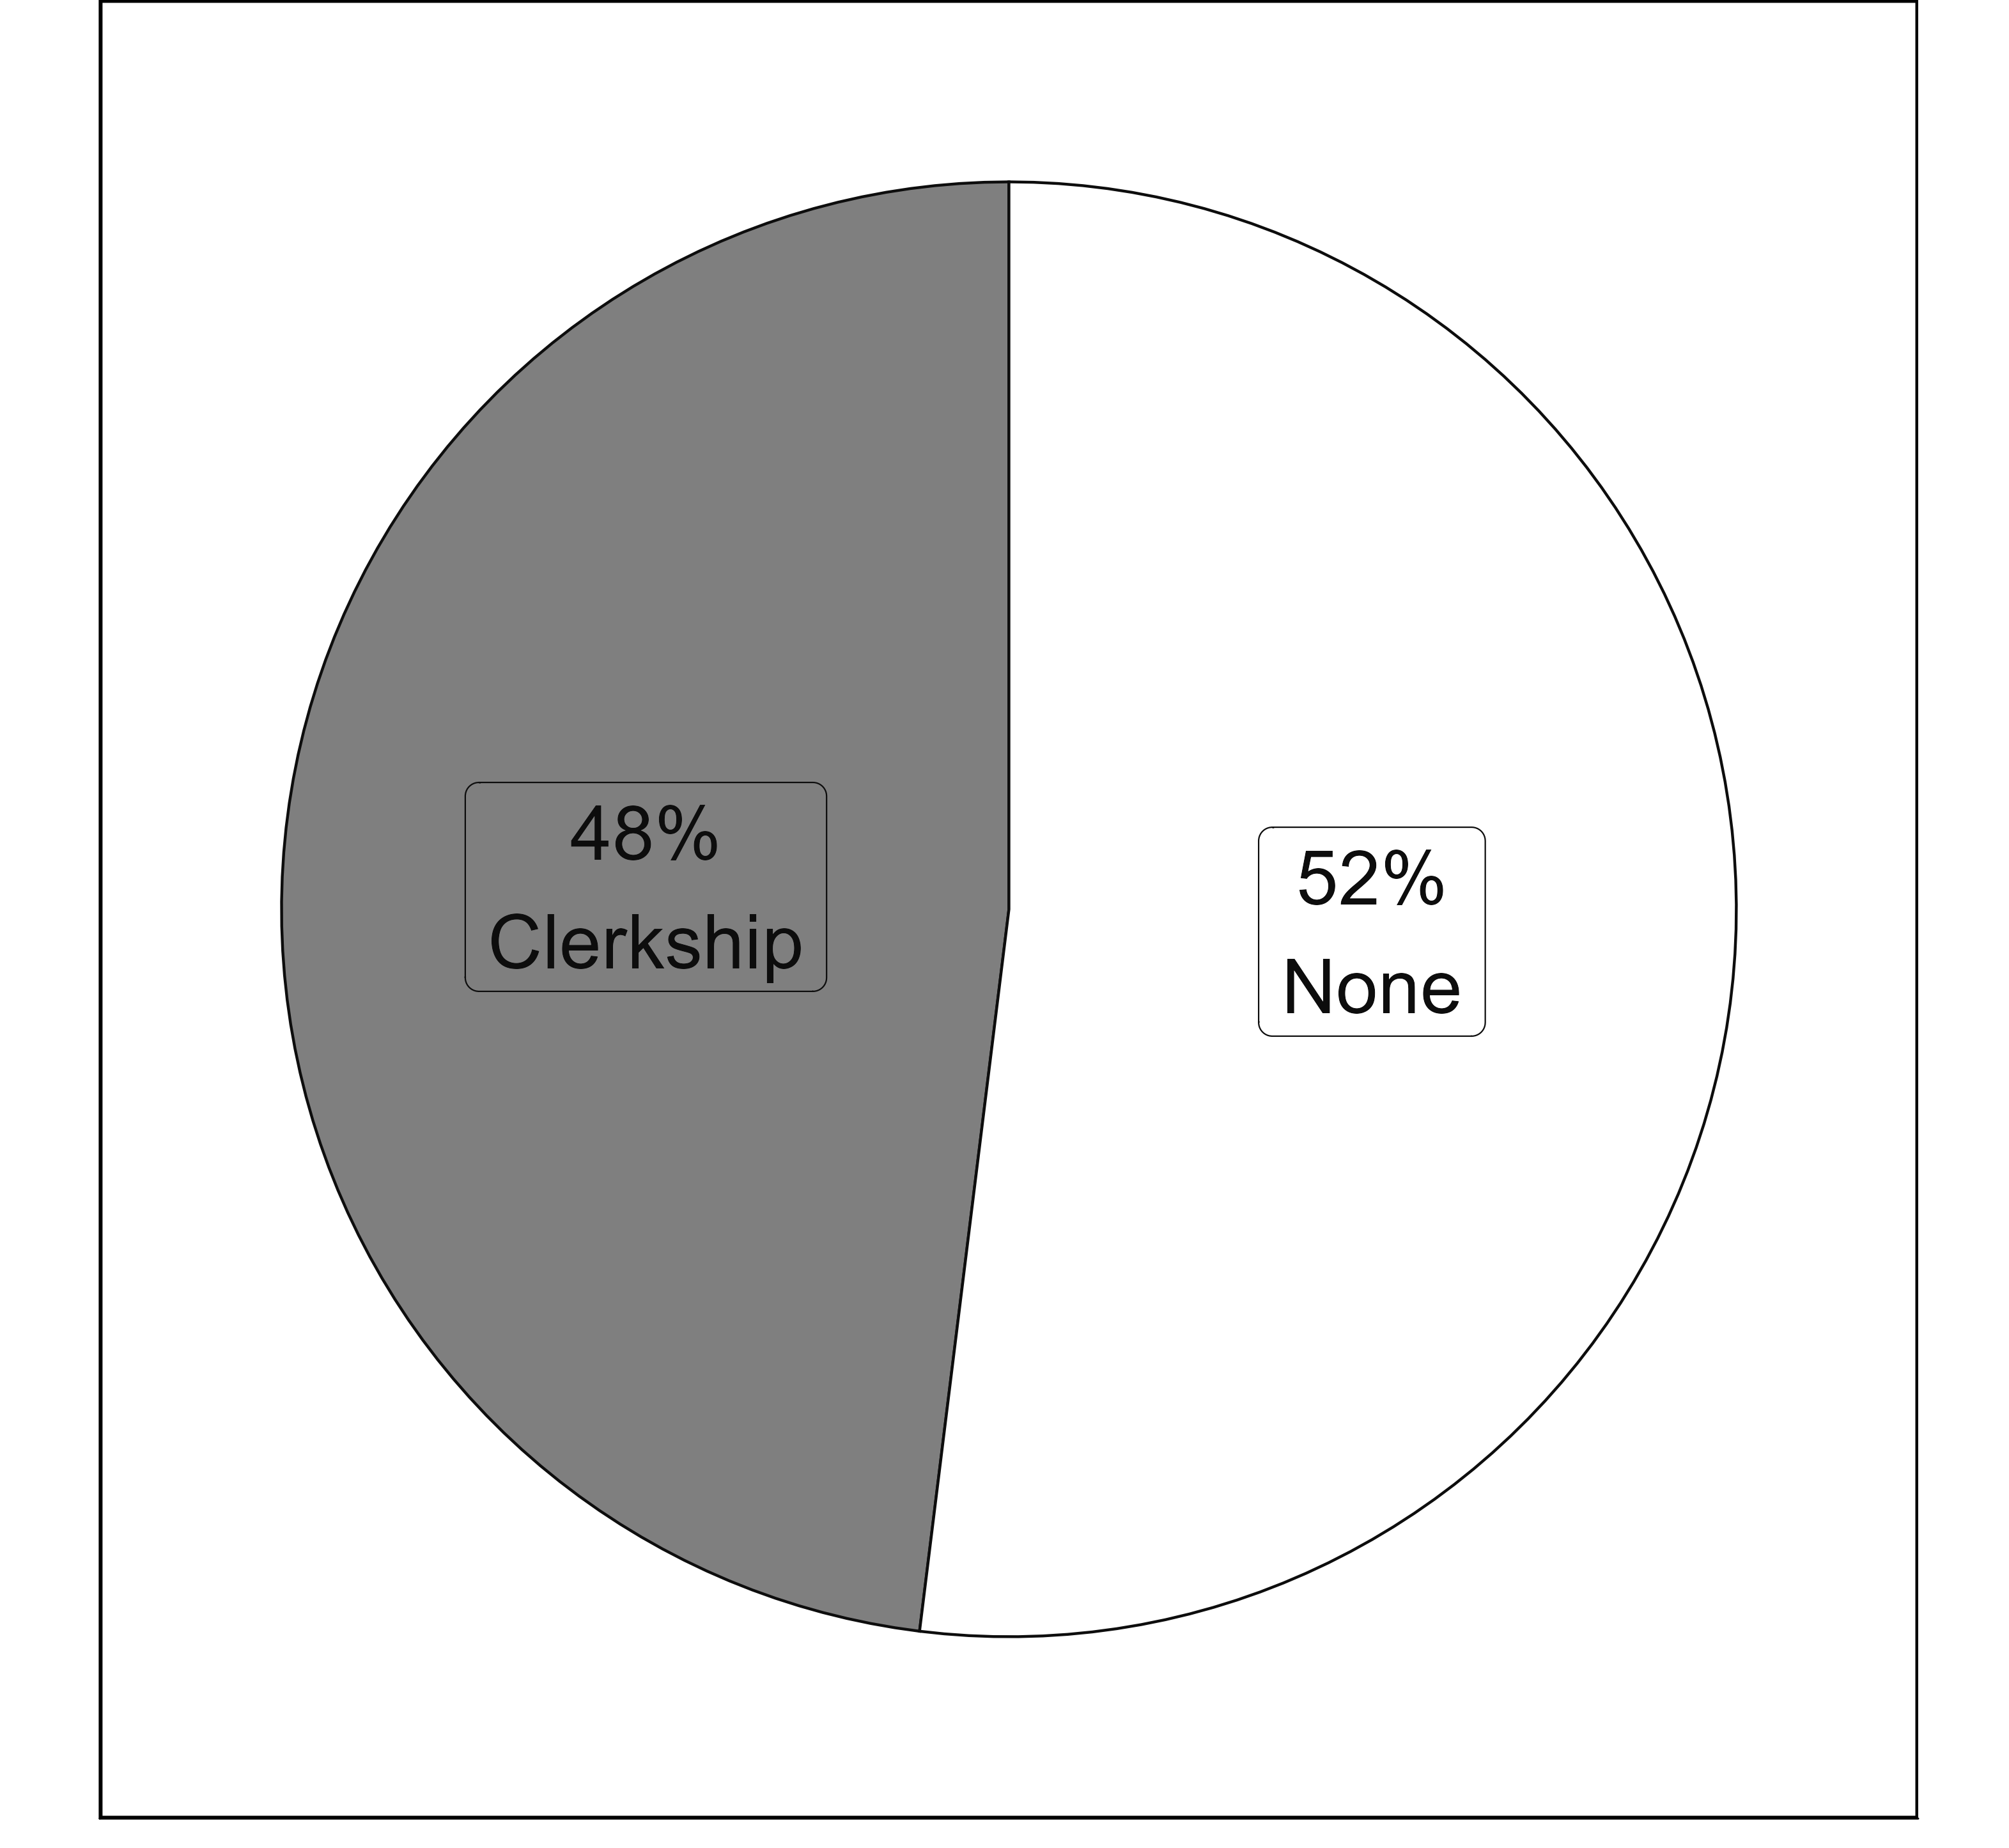
\includegraphics[width=\linewidth]{Figures/statpack_figures/percentage_scotus_clerkship.png}
    \end{figure}

    \begin{figure}[H]
        \centering
        \caption{Attorney Gender}
        \vspace{2.5mm}
        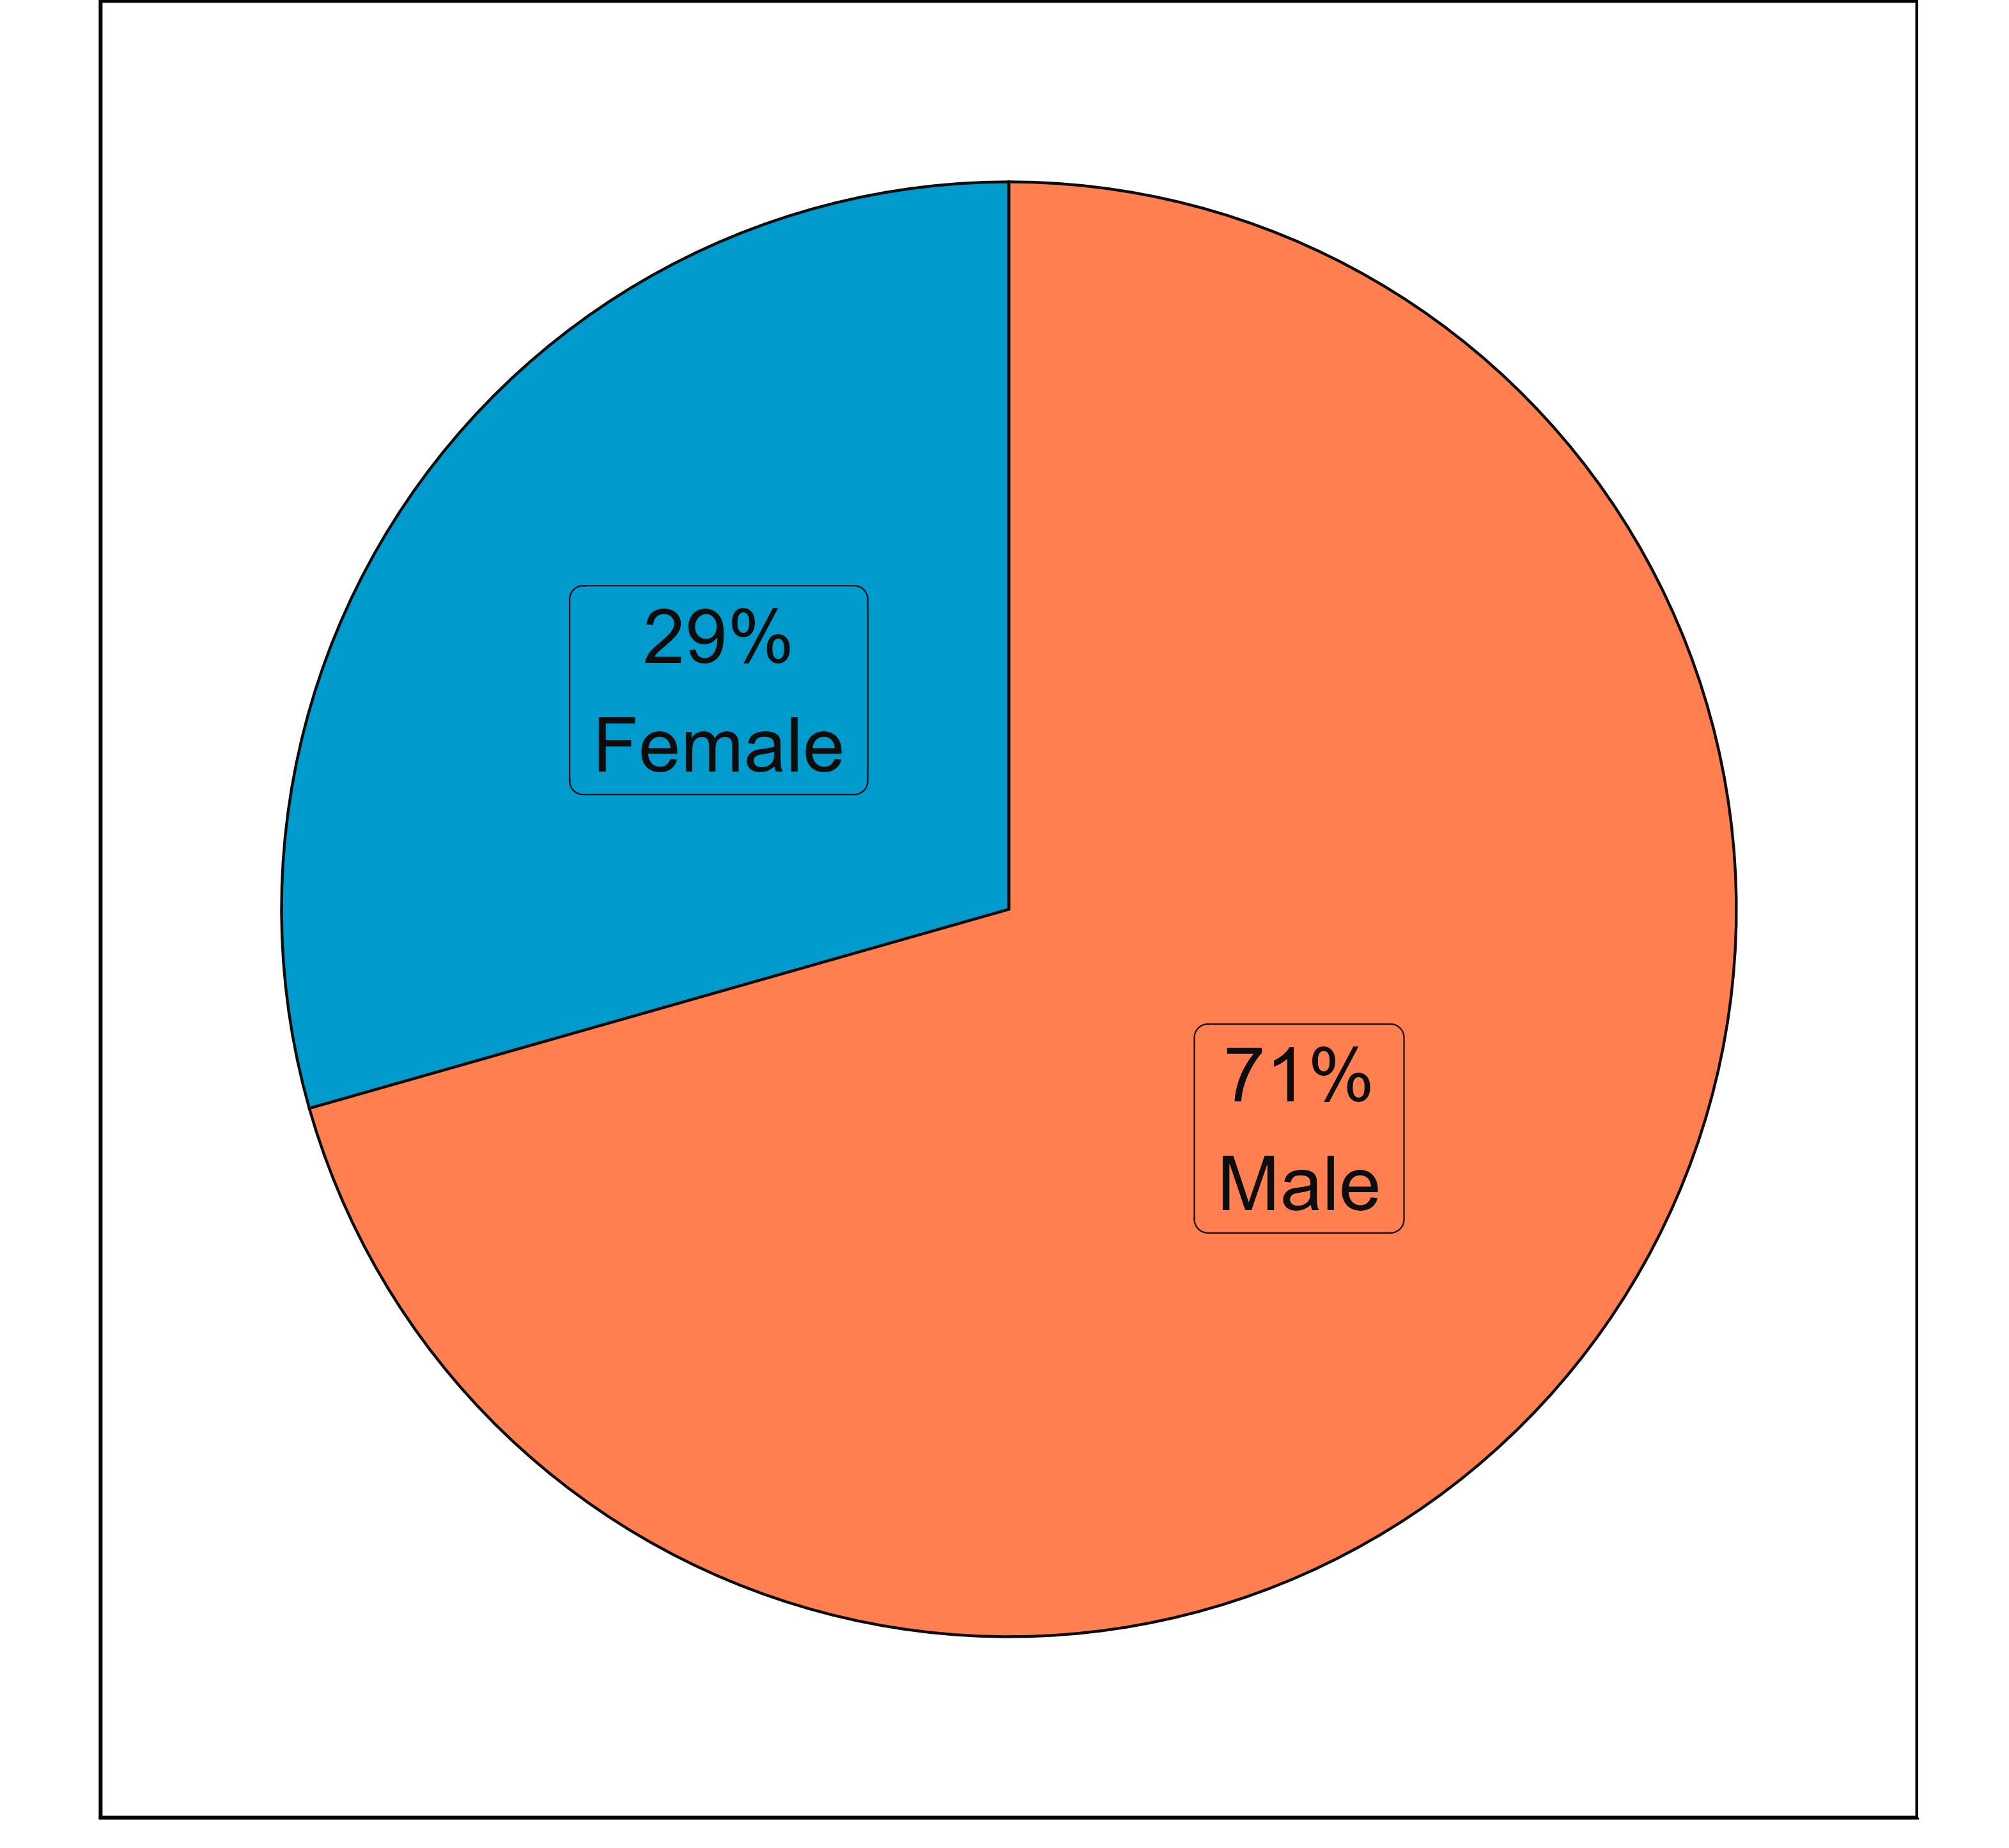
\includegraphics[width=\linewidth]{Figures/statpack_figures/percentage_gender.png}

    \end{figure}

    \begin{figure}[H]
        \centering
        \caption{Experience With the SG's Office}
        \vspace{2.5mm}
        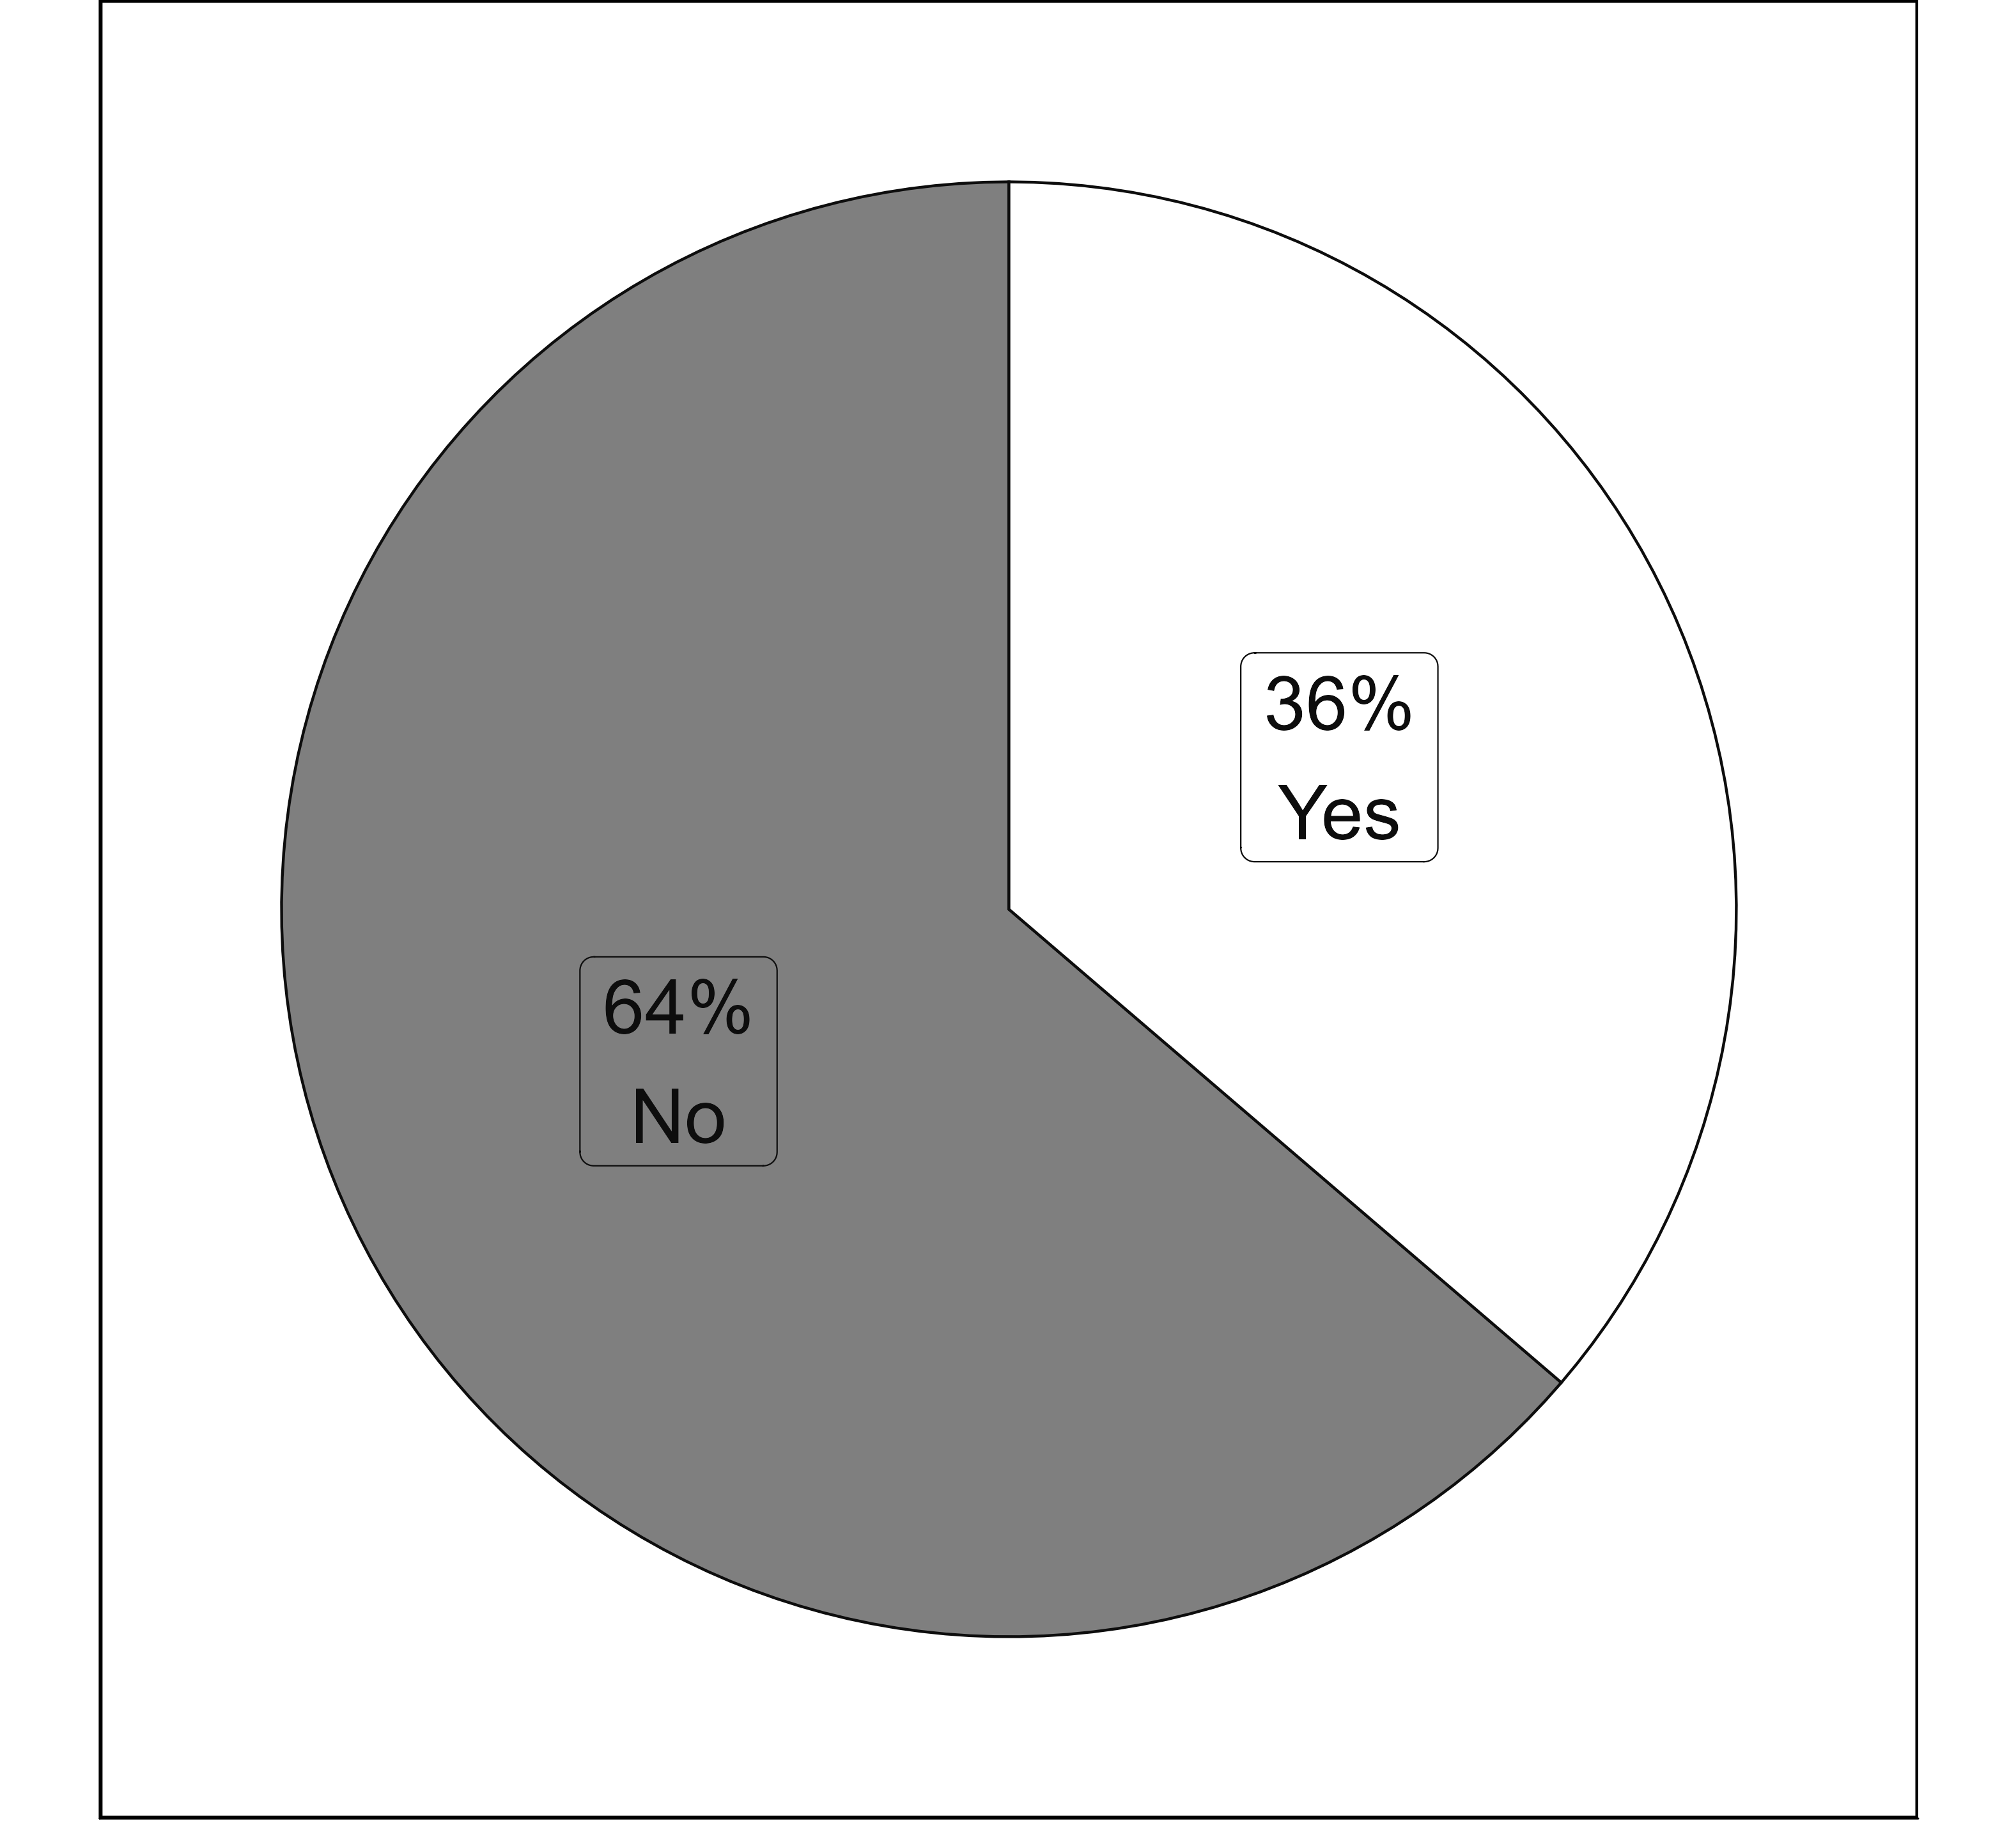
\includegraphics[width=\linewidth]{Figures/statpack_figures/percentage_sg_experience.png}
    \end{figure}
\end{multicols}

\footnotesize{\emph{Note}: Summary information measured using individual attorneys, irrespective of how many times they appeared in oral arguments -- i.e., although (Solicitor) General Elizabeth Prelogar appeared in several arguments during the 2023 Term, they are only referenced as a single observation in the listed attorney statistics.}

\vfill

\end{landscape}

\newpage

\begin{landscape}
\vspace*{\fill}
\begin{figure}[h]
\centering
\caption{Attorney Information (Law School Attendance)}
\vspace{2.5mm}
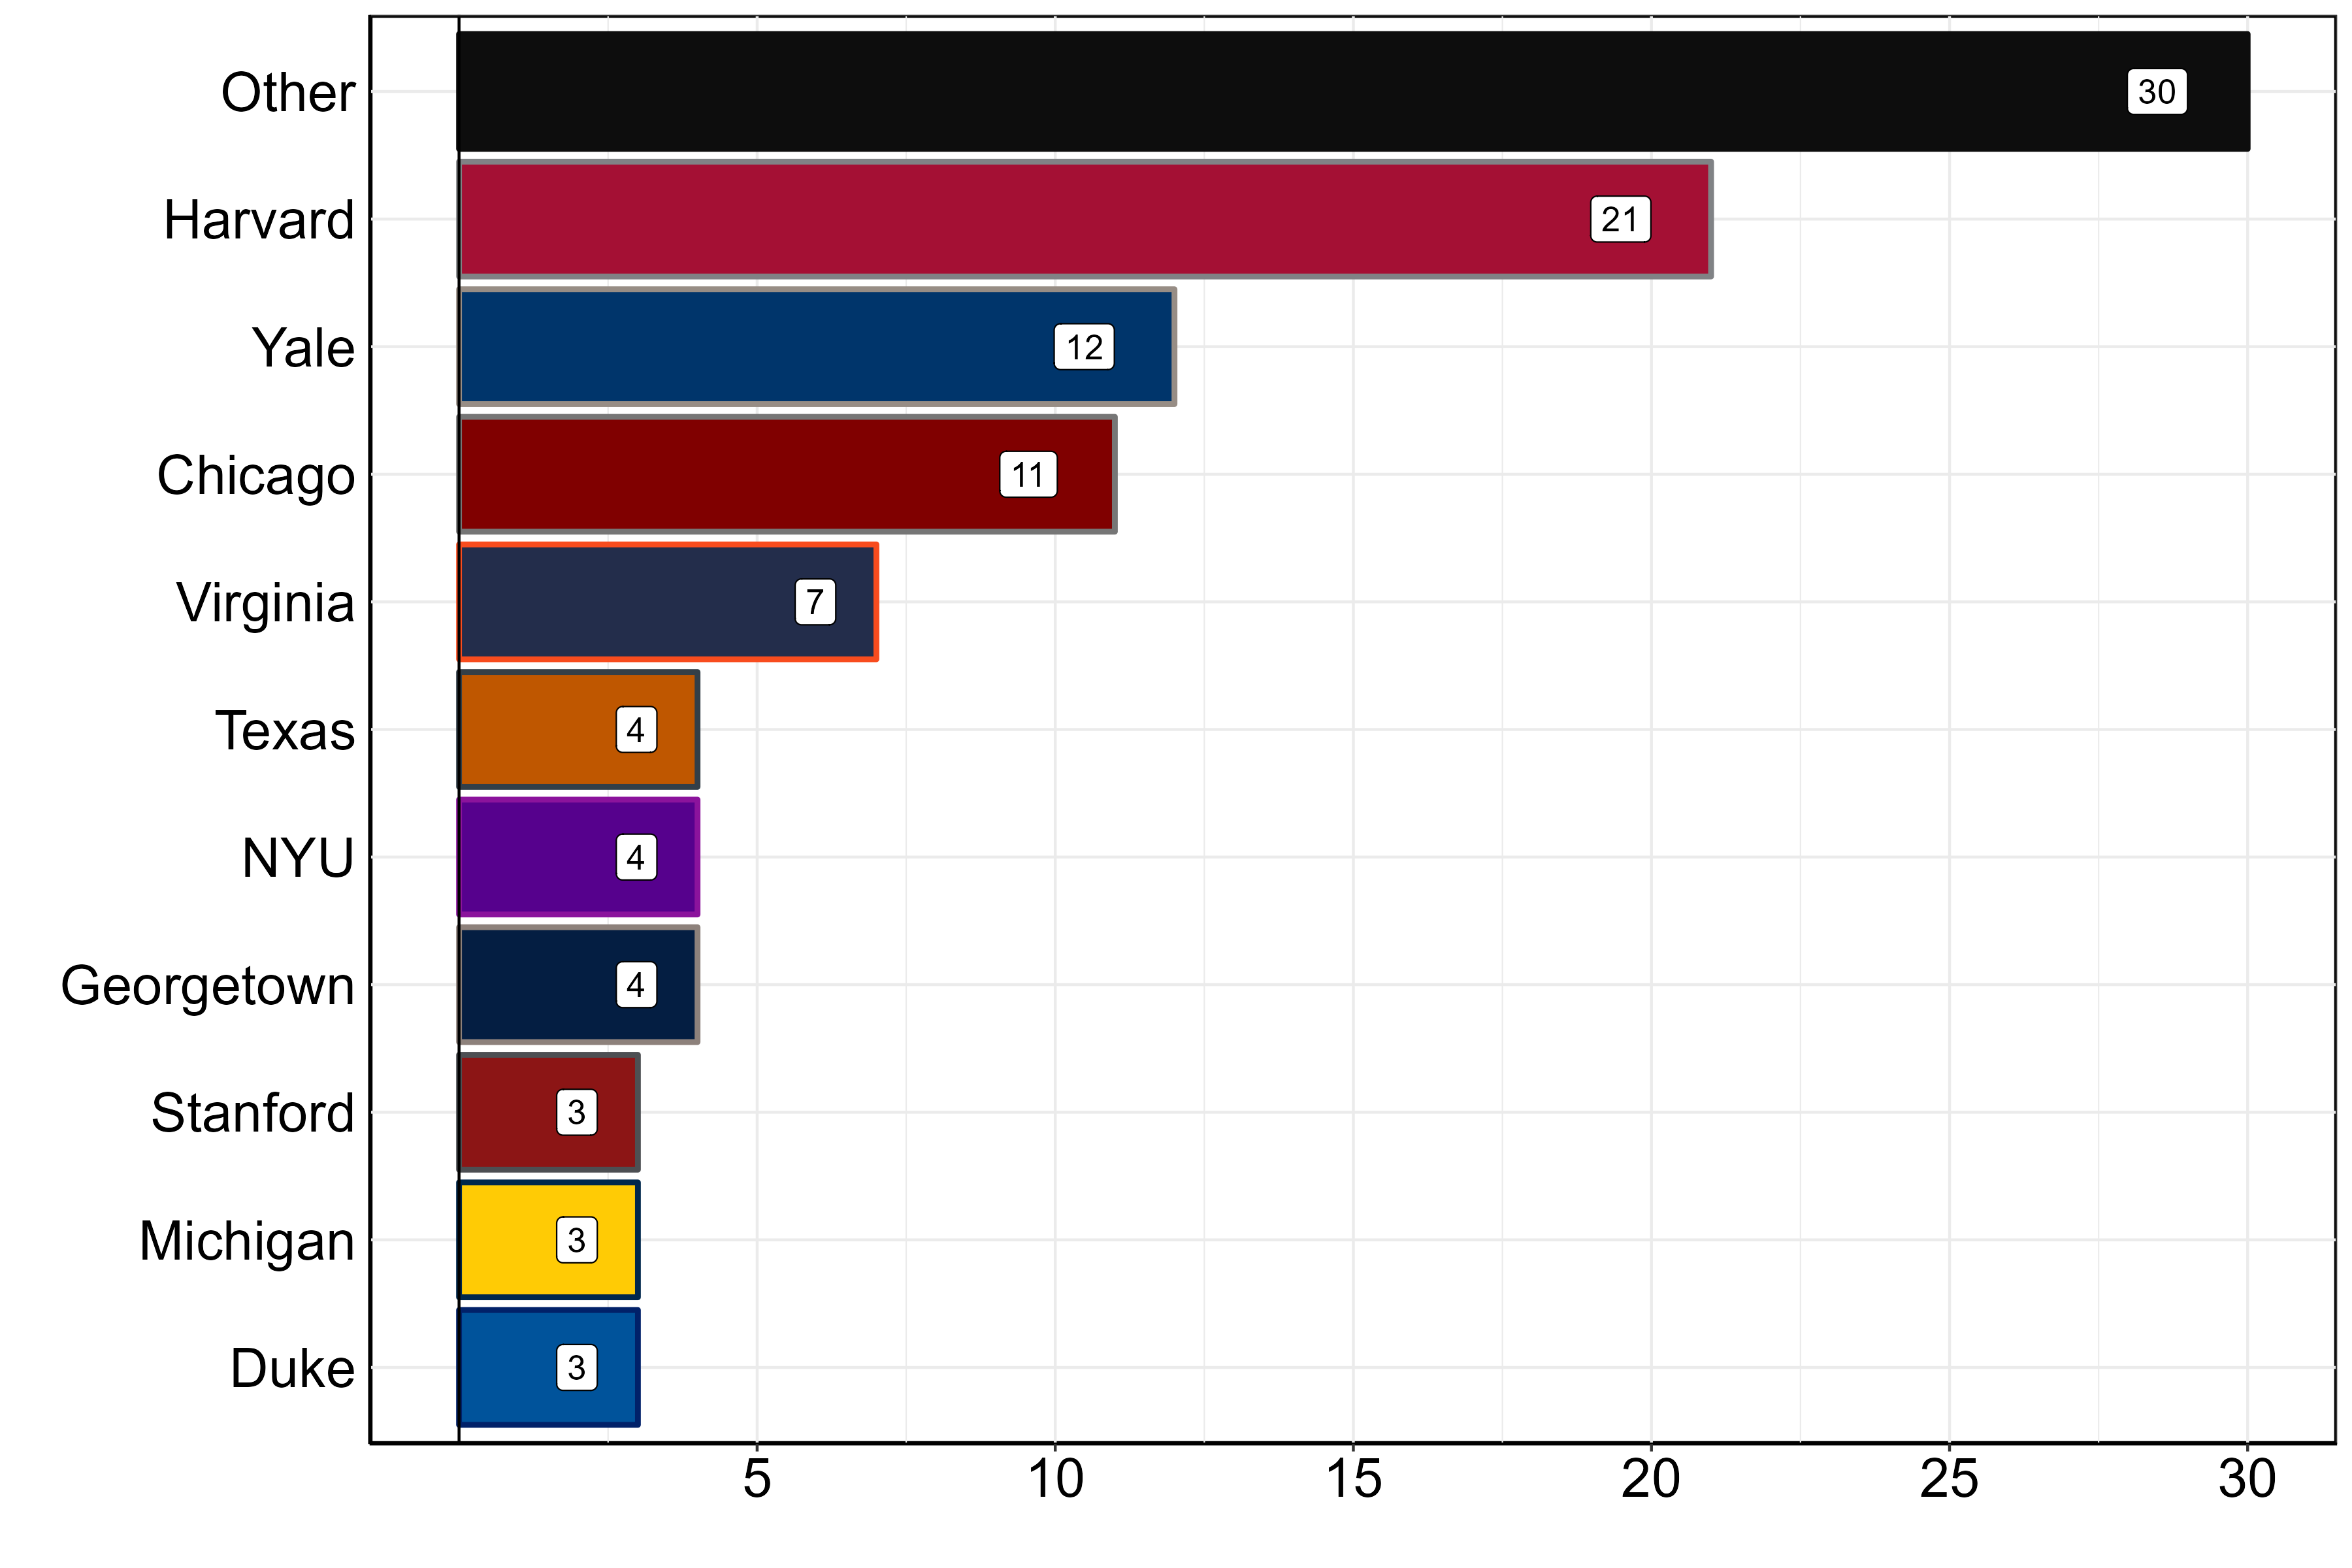
\includegraphics[width=0.95\textwidth]{Figures/statpack_figures/law_school_figure.png} \\
\end{figure}
\vfill
\end{landscape}

\newpage

\begin{landscape}
\vspace*{\fill}
\vspace{2.5mm}
\begin{figure}[h]
\centering
\caption{Attorney Information (SCOTUS Clerkships by Justice)}
\vspace{2.5mm}
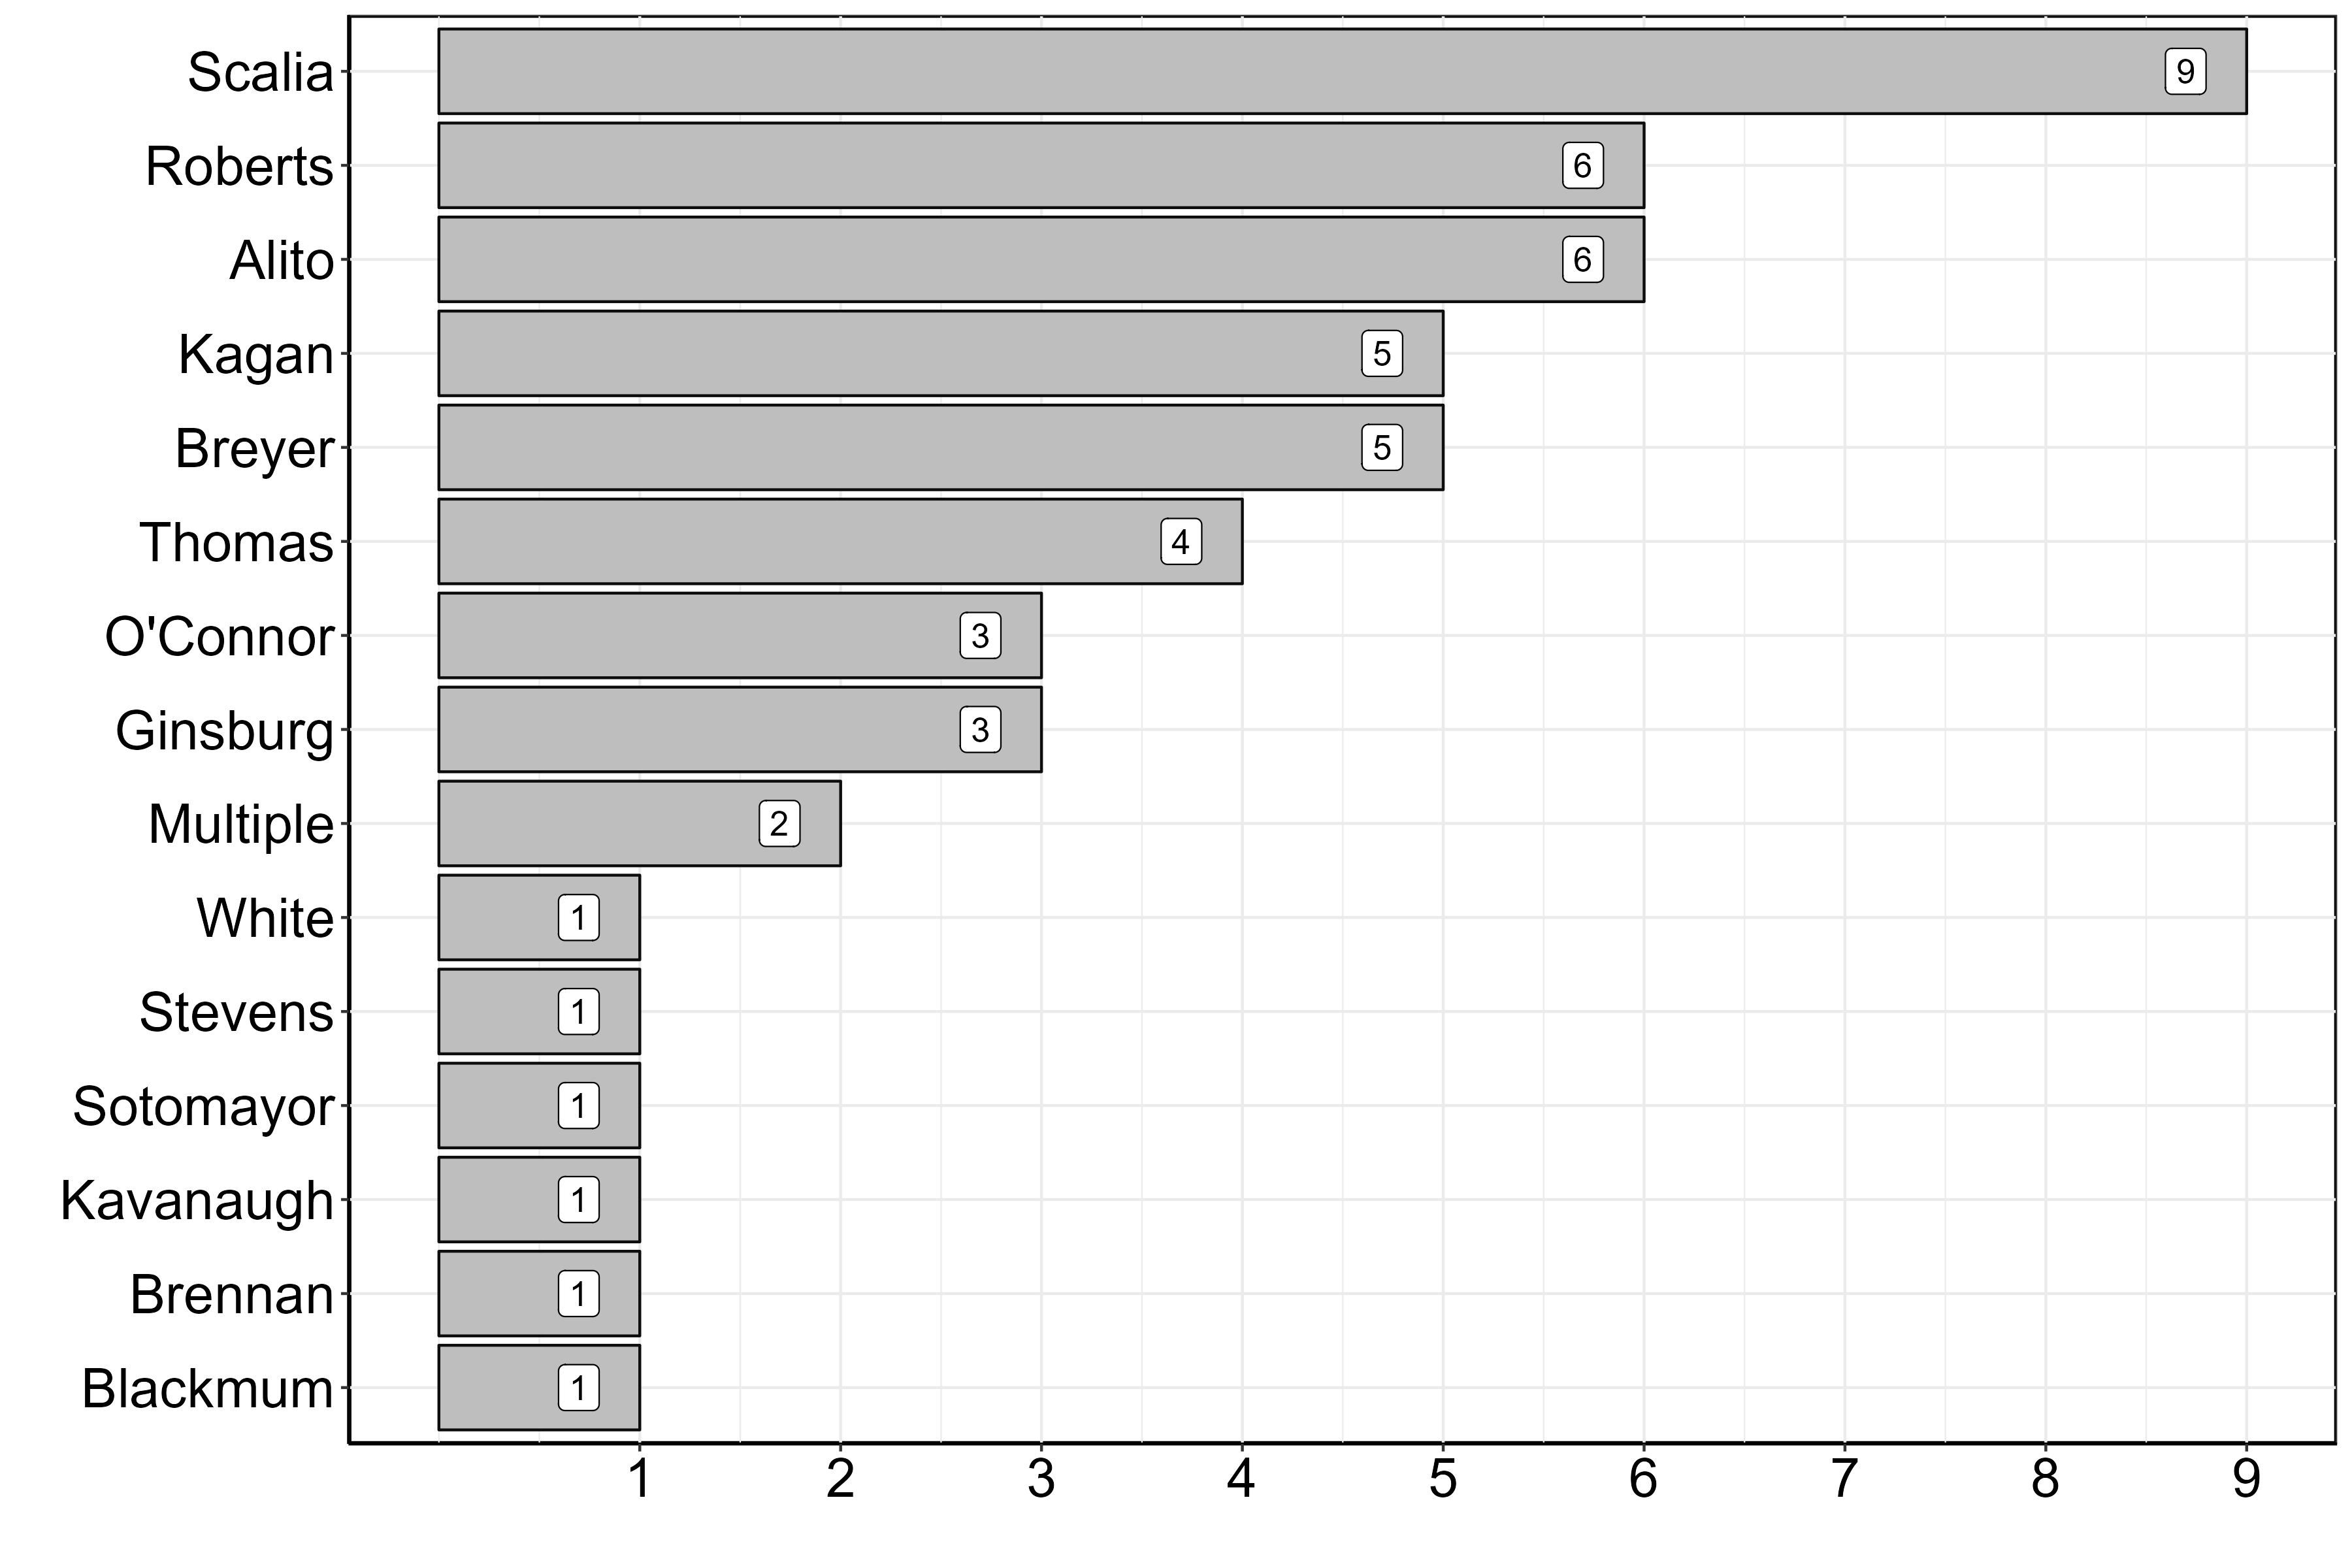
\includegraphics[width=0.95\textwidth]{Figures/statpack_figures/clerkships_by_justice.png} \\
\end{figure}
\vspace{2.5mm}
\footnotesize{\emph{Note}: Elizabeth Prelogar (USSG) and Sopan Joshi both served clerkships with two (\textbf{Multiple}) Justices -- Kagan \& Ginsburg (Prelogar) and Scalia \& Alito (Joshi).}
\vfill
\end{landscape}
